\section{Introduction \& Background}
\subsection{What is MAPF?}
\begin{frame}
    \textbf{What is Multi Agent PathFinding?} \\[1cm]

    \(\blacktriangleright \) Multi-Agent Pathfinding (MAPF) involves planning collision-free paths for multiple agents in a shared environment.

    \(\blacktriangleright \) Various application : warehouse management~\cite{wurman2008coordinating}, video games~\cite{ma2017feasibility}, routing, planning, robotics~\cite{veloso2015cobots}\dots


\end{frame}

\begin{frame}{An example}
    
    \begin{figure}[H]
        \centering
        \caption{Example of Multi agent Pathfinding}
        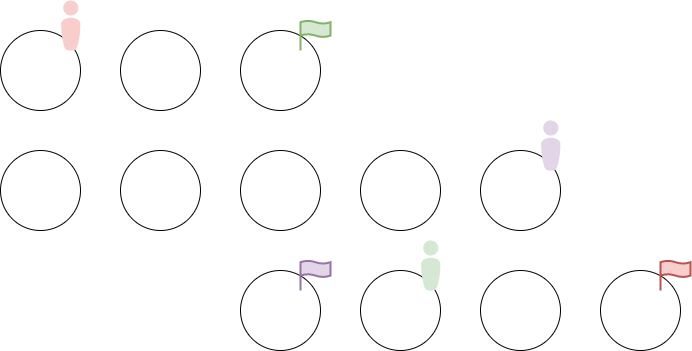
\includegraphics[width=\widthimg]{img/MAPF_example_1.drawio.png}
    \end{figure}

\end{frame}


\begin{frame}{An example}
    
    \begin{figure}[H]
        \centering
        \caption{Example of Multi agent Pathfinding}
        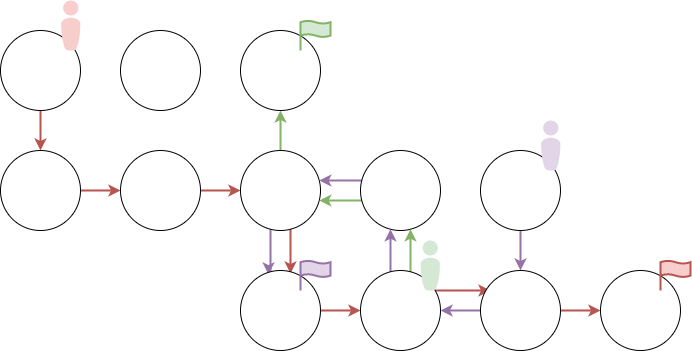
\includegraphics[width=\widthimg]{img/MAPF_example_2.drawio.png}
    \end{figure}

\end{frame}


\begin{frame}{Settings}
    MAPF is defined on a graph.
    
    \begin{block}{Nomenclature}
        \begin{itemize}
            \item The output is a plan \(\Pi\)
            \item \(\Pi\) is a collection of \(\pi\)
        \end{itemize}
    \end{block}
    
    
    \begin{figure}[H]
        \centering
        \caption{Considered conflicts}
        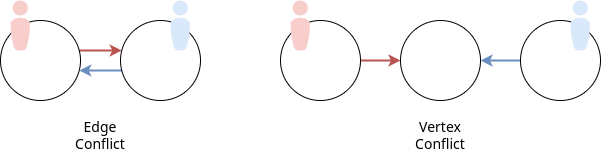
\includegraphics[width=\widthimg]{img/conflict_type.drawio.png}
    \end{figure}


\end{frame}



\subsection{Plan Merging: Motivation, Principle \& Overview}

\begin{frame}{Plan Merging: Motivation, Principle \& Overview}


    \textbf{Principle}
    \begin{itemize}
        \item From path(S) computed without considering conflict
        \item Try to find a conflict free plan out of the previously computed paths
    \end{itemize}


    \textbf{Motivation}
    \begin{itemize}
        \item Computing multiple individual path(s) is not expensive
        \item + Combining them is still faster 
    \end{itemize}


    \textbf{Overview}
    \begin{figure}[H]
        \centering
        \caption{Overview of the process}
        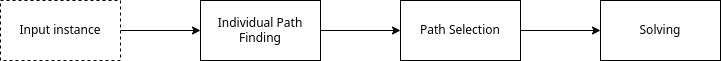
\includegraphics[width=\widthimg]{img/overview.drawio.png}
    \end{figure}
\end{frame}

